\section{Estado del Arte}

En este capítulo se muestran herramientas que logran simular la dinámica orbital y la dinámica de actitud del satélite, además de visualizarlo mediante una interfaz gráfica. Algunos de ellos son simuladores que entregan alguno de los MoP de apuntamiento, así como también softwares especializados en el análisis de budgets de ingeniería, en los cuales se encuentran los SE envelopes descritos.

\subsection{Spacecraft Control Toolbox}

Spacecraft Control Toolbox (SCT) para MATLAB le permite diseñar, analizar y simular naves espaciales. Este producto es utilizado en todo el mundo por organizaciones líderes en investigación y desarrollo y fabricantes de naves espaciales. Se proporcionan más de dos mil funciones para dinámica, simulación, análisis y diseño de actitud y órbita. Puedes construir un satélite utilizando las herramientas gráficas CAD; diseñar y analizar los sistemas de control; realizar análisis de perturbaciones y pruebe el sistema de control en una simulación de seis grados de libertad, todo en el lenguaje de programación MATLAB \cite{ref18}. Existen tres módulos disponibles, los cuales se muestran a continuación:

\begin{itemize}
	\item \textit{CubeSat Toolbox}: Es el producto más básico disponible, a un costo de 495 dólares. Está diseñado para CubeSat específicamente y sus principales características son el modelamiento de la dinámica y control de actitud (perturbaciones, controladores PID en conjunto con actuadores), propagación de orbita, cambios de marco de referencia, visualización (2D y 3D) y planeamiento de la misión. En la Figura~\ref{fig:cube_Tool}, se presenta un resumen de los datos obtenidos por el simulador una vez creado el diseño 3D en CAD. Por otro lado, en la Figura~\ref{fig:cube_ctrl}, se muestra en específico la ventana de control del simulador, mostrando tanto los cuaterniones de rotación, como los torques y las razones de cambio de la rueda de reacción montada en el CubeSat.
	
	\begin{figure}[H]
		\centering    
		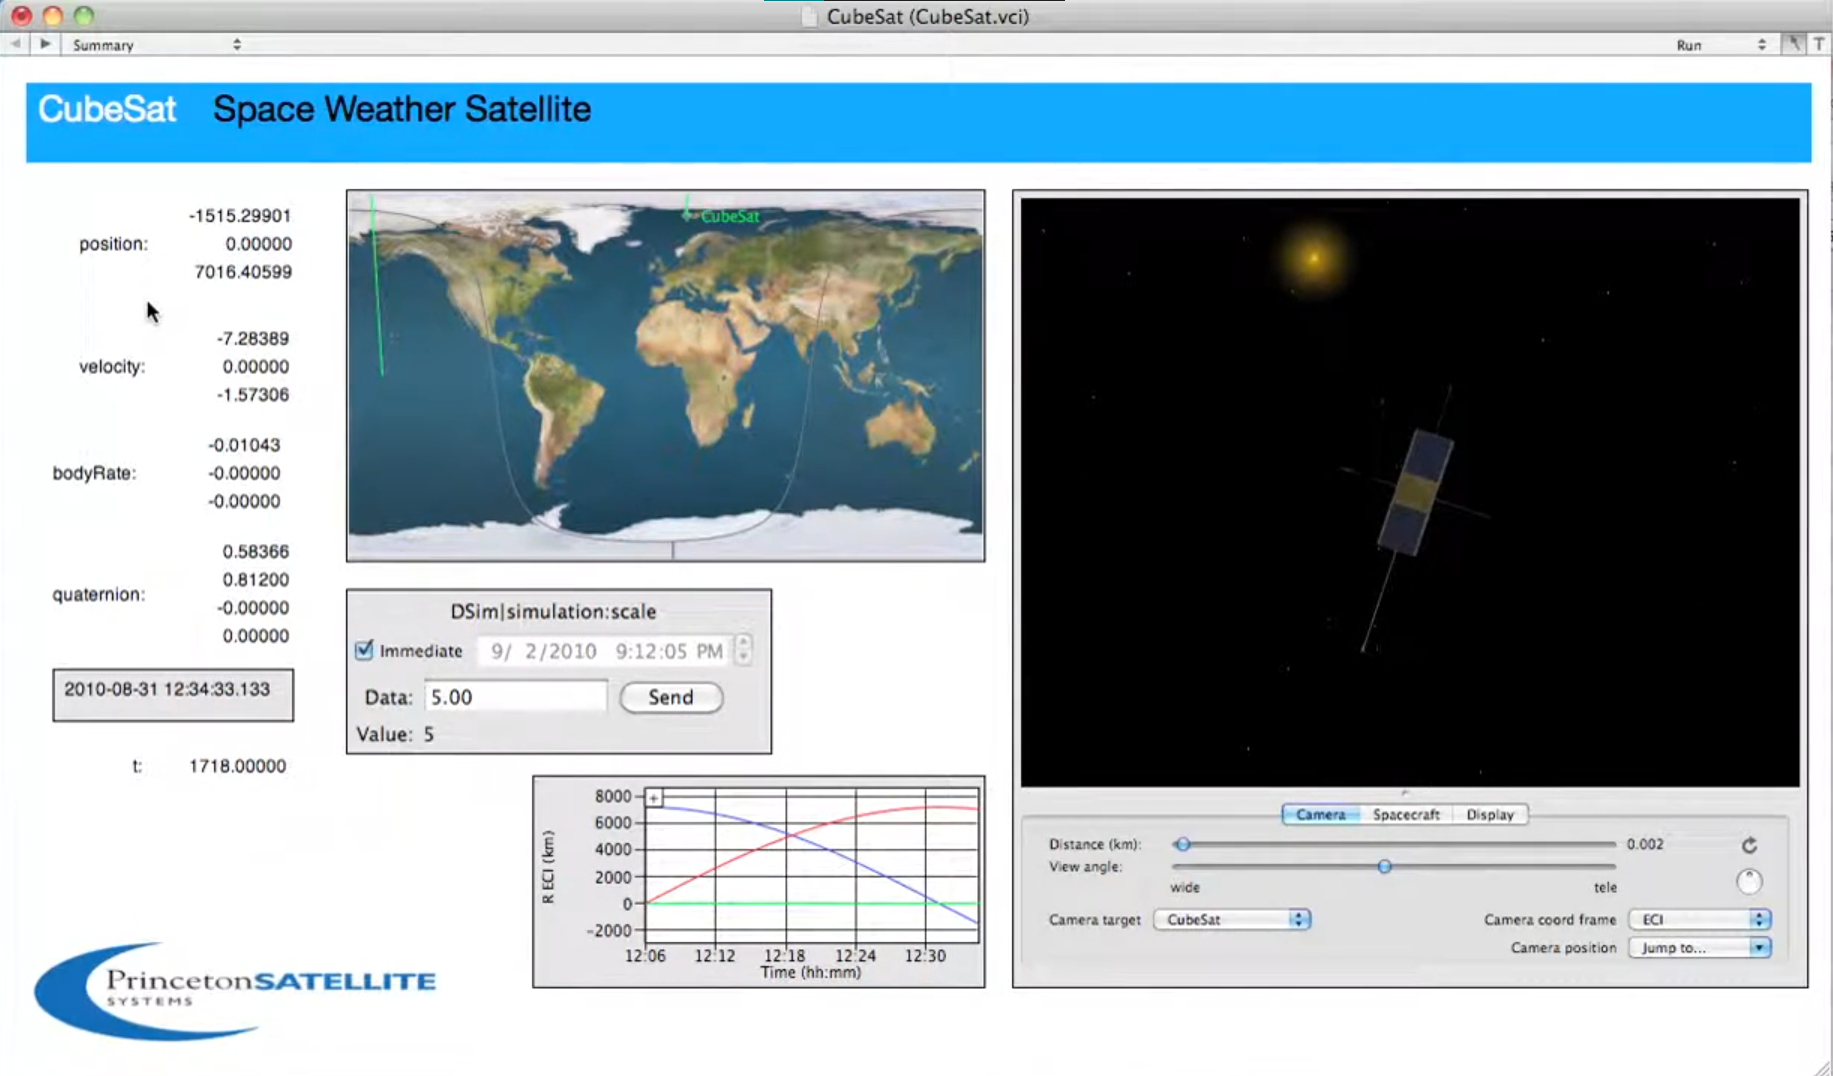
\includegraphics[width=0.75\textwidth]{Cubesat_Toolbox.png}
		\caption{Resumen de la dinámica orbital y de actitud del satélite en CubeSat Toolbox.}
		\label{fig:cube_Tool}
	\end{figure}
	
	\begin{figure}[H]
		\centering    
		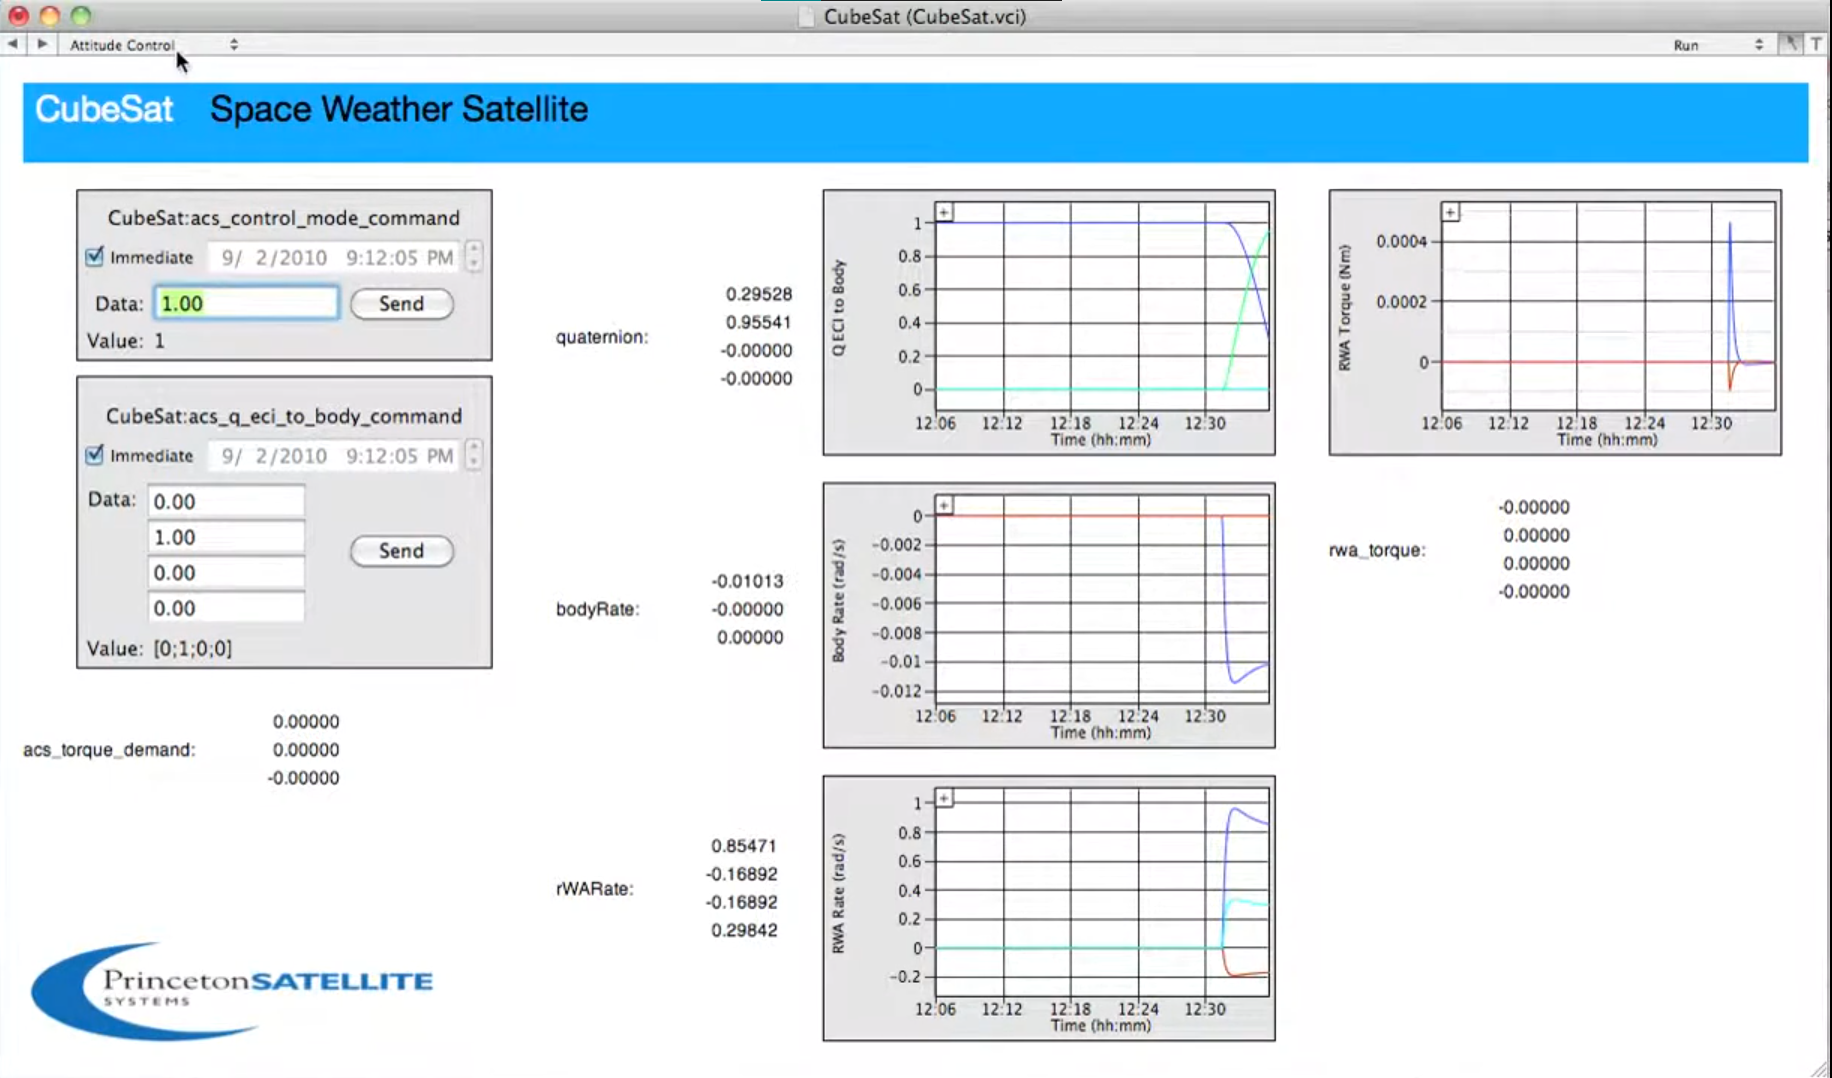
\includegraphics[width=0.75\textwidth]{Cubesat_Toolbox_2.png}
		\caption{Ventana de control del simulador de un CubeSat en CubeSat Toolbox.}
		\label{fig:cube_ctrl}
	\end{figure}
	
	\item \textit{Spacecraft Control Toolbox versión académica}: La edición académica de la caja de herramientas contiene gran parte del software profesional Spacecraft Control Toolbox, incluidas las herramientas CAD, las funciones de diseño de control y dinámica de actitud, la mecánica orbital y el módulo CubeSat. Además, incluye esquemas de apuntamiento según marcos de referencia LVLH, sun-nadir pointing y latitude/longitude, y también otorga los pointing budgets más relevantes como la exactitud de apuntamiento. Esta versión cuesta 3995 dólares su adquisición y presenta un breve tutorial en el canal de YouTube de Princeton.
	
	\item \textit{Spacecraft Control Toolbox versión profesional}: La edición profesional de Spacecraft Control Toolbox ofrece todo lo que hay en las versiones CubeSat y Academic, con la adición de herramientas avanzadas para la estimación de actitud y órbita, modelado de sensores y actuadores y análisis de subsistemas. Las aplicaciones de la caja de herramientas incluyen diseño de sistemas de control, simulación no lineal, análisis de órbitas y planificación de misiones, incluidas trayectorias interplanetarias, diseño y disposición de naves espaciales, estudios comerciales y visualización de actitudes y órbitas. La versión profesional cuesta 11995 dólares, siendo esta la más completa y a la vez más cara entre las tres mencionadas.
\end{itemize}


\subsection{Ansys Systems Tool Kit (STK)}

STK es una plataforma de software líder en el mercado diseñada para el modelado y análisis de sistemas complejos y sus interacciones en una variedad de dominios, incluyendo espacio, defensa y aplicaciones aeroespaciales. Esta herramienta proporciona una serie de capacidades avanzadas que permiten a los ingenieros, científicos y analistas modelar, simular y visualizar sistemas dinámicos de manera efectiva \cite{ref34}.

Es relevante ya que es capaz de modelar un satélite mediante su diseño 3D, mostrando gráficamente como este se propaga a través de la órbita. También es capaz de simular los cambios de actitud del satélite a través del tiempo y mostrar si efectivamente se está apuntando hacia la zona requerida de la tierra (exactitud de apuntamiento). En la Figura~\ref{fig:STK} se aprecia una imagen referencial de la simulación de un satélite en 3D y sus marcos de referencia cuerpo y LVLH. El costo de la licencia investigativa de este software es de alrededor de 4527 dólares por un año, que sería la versión útil para la realización del proyecto.

\begin{figure}[H]
	\centering    
	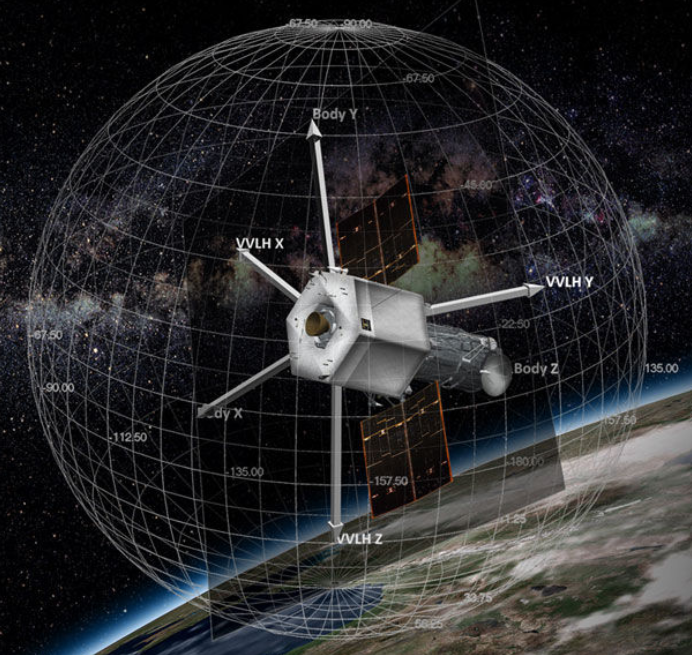
\includegraphics[width=0.4\textwidth]{STK.png}
	\caption{Imagen referencial de STK para simulación de un satélite.}
	\label{fig:STK}
\end{figure}
\subsection{Aerospace Blockset}

Dentro de este módulo en MATLAB, existen librerías capaces de modelar, simular y analizar CubeSats con facilidad \cite{ref19}. Algunas de las capacidades clave incluyen:

\begin{itemize}
	\item \textit{Modelado de CubeSats}:  El modelo de plantilla es un ejemplo listo para simular que contiene un bloque de vehículo CubeSat. MATLAB permite a los usuarios modelar CubeSat para proporcionar una opción de planificación de misión de alto nivel/creación rápida de prototipos para modelar y propagar rápidamente órbitas de satélites, un satélite a la vez. En este bloque se debe especificar el estado orbital inicial y modo de control de actitud (apuntamiento hacia el sol, nadir Tierra o personalizado), como se observa en la Figura~\ref{fig:blockset_1}.
	
	\begin{figure}[H]
		\centering    
		\includegraphics[width=0.7\textwidth]{blockset_1.png}
		\caption{Plantilla de Simulink para el diseño de un CubeSat.}
		\label{fig:blockset_1}
	\end{figure}
	
	\item Simulación de Misiones: El proyecto es un ejemplo listo para simular con visualización utilizando Simulink 3D Animation, como se muestra en la Figura~\ref{fig:blockset_2}jemplo utiliza un subsistema de modelo de vehículo por defecto, pero también se puede utilizar el modelo de CubeSat diseñado en el paso anterior. Con el módulo, es posible simular misiones completas de CubeSats, lo que incluye la evaluación de la trayectoria, la dinámica orbital con modelos de perturbaciones incluidas y las operaciones a bordo. Esto es esencial para prever el comportamiento del CubeSat en el espacio y optimizar su rendimiento.
	
	\begin{figure}[H]
		\centering    
		\includegraphics[width=0.9\textwidth]{blockset_2.png}
		\caption{Plantilla de Simulink para la modelación y simulación del CubeSat en base a la visualización en Simulink 3D.}
		\label{fig:blockset_2}
	\end{figure}	
	
	\item \textit{Proyecto de ingeniería de sistemas basados en modelos (MBSE) en CubeSat}: Es un ejemplo listo para simulación que muestra cómo modelar la arquitectura de una misión espacial con System Composer y Aerospace Blockset. El proyecto hace referencia al Proyecto de simulación CubeSat para reutilizar modelos de subsistema, luego agrega una capa de arquitectura System Composer, vincula los requisitos del sistema con los componentes de la arquitectura y verifica los requisitos de la misión de nivel superior con Simulink Test™. El proyecto visualiza los resultados utilizando Simulink 3D Animation, escenarios satelitales de Aerospace Toolbox y Mapping Toolbox™. Todo esto se muestra según los bloques mostrados en la Figura~\ref{fig:blockset_3}.
	
	\begin{figure}[H]
		\centering    
		\includegraphics[width=0.6\textwidth]{blockset_3.png}
		\caption{Visualización del MBSE de CubeSat.}
		\label{fig:blockset_3}
	\end{figure}	
	
	Mediante la última librería mencionada se puede obtener la observación terrestre de un CubeSat, además de visualizar los budgets de costo como lo es el precio, la masa, la potencia tanto peak como promedio y el tamaño. También presenta en una interfaz gráfica los errores de determinación de actitud y de apuntamiento, además de los torques ejercidos por los actuadores (sean modelados o por defecto dentro del programa), como se muestra en la Figura~\ref{fig:blockset_4}. Así, se puede visualizar el resultado como muestra la Figura~\ref{fig:blockset_5}.
	
	\begin{figure}[H]
		\centering    
		\includegraphics[width=0.6\textwidth]{blockset_4.png}
		\caption{Perfil de CubeSat según los SE envelopes configurables.}
		\label{fig:blockset_4}
	\end{figure}	
	
	\begin{figure}[H]
		\centering    
		\includegraphics[width=0.75\textwidth]{blockset_5.png}
		\caption{Simulación de apuntamiento de la Tierra hacia la estación terrestre.}
		\label{fig:blockset_5}
	\end{figure}	
\end{itemize}

\subsection{Valispace}

Valispace es una plataforma integral de ingeniería y gestión de proyectos diseñada para simplificar y optimizar el proceso de desarrollo de productos y sistemas, especialmente en industrias como la aeroespacial. La plataforma ofrece una variedad de herramientas y características poderosas que permiten a los equipos de ingeniería colaborar eficientemente, gestionar requisitos y parámetros críticos, y tomar decisiones informadas en tiempo real \cite{ref35}.

Las características claves son la gestión de datos en tiempo real, permitiendo el acceso en tiempo real y la colaboración de los miembros del equipo de ingeniería de forma actualizada. También permite a los equipos diseñar, analizar y optimizar sistemas de ingeniería complejos en base a requisitos que se imponen en el mismo programa al inicio del proyecto. Además, Valispace facilita el cálculo de parámetros críticos como costos, masa, potencia y tamaño, lo que es esencial en proyectos de ingeniería. Los resultados se pueden calcular y actualizar automáticamente a medida que se realizan cambios en el diseño.

\subsection{Basilisk}

El simulador Basilisk es un entorno de simulación avanzado, modular y extensible, desarrollado principalmente por el Laboratorio de Sistemas de Vehículos Espaciales de la Universidad de Colorado, Boulder. Su principal objetivo es facilitar la simulación de sistemas de naves espaciales, con un enfoque en la dinámica y el control de actitud. Este simulador ha sido ampliamente utilizado en investigaciones académicas y proyectos que requieren la modelación precisa de la dinámica y control de vehículos espaciales \cite{ref36}.

Una de las principales ventajas de Basilisk es su capacidad para simular sistemas multi-plataforma y multi-cuerpo, permitiendo la modelación de la dinámica orbital y de actitud de diversos cuerpos en el espacio. Esto incluye la simulación de perturbaciones ambientales, así como el comportamiento de subsistemas complejos como el ADCS (Attitude Determination and Control System). Estas capacidades hacen que Basilisk sea especialmente útil para misiones que involucran satélites pequeños o CubeSats, donde las dinámicas precisas y los ajustes de actitud son críticos.

Otra de las fortalezas del simulador radica en su arquitectura modular. Cada subsistema —como los sensores, actuadores, o la dinámica orbital— está diseñado de manera independiente, lo que permite no solo la fácil personalización del código, sino también la posibilidad de integrar nuevos módulos o realizar simulaciones específicas de determinados componentes. Esta flexibilidad es clave para proyectos de investigación que requieren ajustes finos y configuraciones personalizadas.

El simulador también ofrece la capacidad de realizar simulaciones tanto en tiempo real como en tiempo no real, lo que resulta útil para diferentes tipos de aplicaciones. Las simulaciones en tiempo real permiten la implementación de pruebas de hardware-in-the-loop, mientras que las simulaciones en tiempo no real ofrecen mayor fidelidad para estudios más detallados.

\subsection{Resumen de los simuladores disponibles}

Para tener en claro si es posible el uso de algunos de estos softwares presentes en el estado del arte (SOA) en la suite de simulación, se toma en cuenta la Tabla~\ref{tab:sims}, en la cual, en base a criterio propios, se analiza cada opción y su viabilidad.

\begin{table}[ht]
	\centering
	\caption{Comparativa de software/simuladores para CubeSats.}
	\label{tab:sims}
	\begin{tabular}{|l|c|c|c|c|}
		\hline
		\textbf{Software/} & \textbf{Precio [USD]}  & \textbf{Dificultad} & \textbf{MoP de} & \textbf{SE envelopes} \\
		\textbf{simulador} &  &  & \textbf{apuntamiento} &  \\ \hline
		\textit{CubeSat}     & 495 + Matlab          & Media               & No presenta                & Potencia                \\ 
		\textit{Toolbox}     & & &  &            \\ \hline
		SCT                 & 3995 + Matlab         & Alta                & Exactitud   & Potencia          \\ 
		académico                & &  &  de apuntamiento & y masa          \\ \hline
		SCT               & 11995 + Matlab        & Alta                & Exactitud de & Potencia, \\
		profesional              &  &  &  apuntamiento/agilidad & masa y tamaño \\ \hline
		\textit{Aerospace}  & Matlab                & Muy             & Exactitud de   & Todos, con imposición \\
		\textit{Blockset}  &                 & alta            &  apuntamiento  & de requisitos \\ \hline
		Systems               & 4527 por año          & Media               & Exactitud de  & Potencia         \\ 
		ToolKit              & &                & apuntamiento/agilidad &          \\ \hline
		Valispace                    & 1295 por año          & Media               & No presenta                & Todos                  \\ \hline
		Basilisk & Gratis & Muy Alta & Configurable & Configurable \\ \hline
	\end{tabular}

\end{table}


Para el caso del precio, son accesibles las opciones de CubeSat Toolbox y Aerospace Blockset, ya que una suscripción de MATLAB cuesta alrededor de 275 USD por año para versión académica, la cual se presenta disponible en el marco de su uso dentro de la Universidad de Concepción como estudiante/académico. Se descarta la primera opción al no presentar un análisis de los MoP de apuntamiento. Otra razón para descartar su uso es que se presenta exclusivamente en MATLAB, siendo que la suite de simulación se pretende armar en Python, por lo que habría que reformular el código dentro de este lenguaje de programación. 

Por otro lado, el Aerospace Blockset se presenta como una buena opción, aunque sea un pack de herramientas disponibles en MATLAB. Si bien esta logra analizar al menos uno de los MoP de apuntamiento, su uso se basa en MBSE, el cual requiere de un manejo del Systems Engineering de medio a alto, escapándose en parte del conocimiento requerido para la optimización de los resultados en el simulador. Además, no presenta la opción de hacer lazo cerrado por fuera del software, por lo que la combinación de herramientas es bastante rígida.

Finalmente, Basilisk se muestra como una opcion interesante a considerar, ya que presenta ya simulado la dinamica orbital y de actitud considerando distinto hardware del ADCS. Esta se toma en cuenta solo como una buena referencia, debido a su elevada curva de aprendizaje y a su documentación que puede ser demasiado técnica o incompleta para el tiempo acotado de trabajo. Además, aunque se pueden realizar simulaciones detalladas del sistema ADCS y dinámicas orbitales, Basilisk no tiene un enfoque nativo en la optimización de sistemas, teniendo que configurar los parametros de rendimiento y costo para este uso.

Por lo tanto, de los simuladores que se pueden adquirir, sirven como una base para implementar de manera propia una suite de simulación con capacidad de optimización.